\chapter{Implementacija i korisničko sučelje}
		
		
		\section{Korištene tehnologije i alati}
		
			%\textbf{\textit{dio 2. revizije}}
			
			 %\textit{Detaljno navesti sve tehnologije i alate koji su primijenjeni pri izradi dokumentacije i aplikacije. Ukratko ih opisati, te navesti njihovo značenje i mjesto primjene. Za svaki navedeni alat i tehnologiju je potrebno \textbf{navesti internet poveznicu} gdje se mogu preuzeti ili više saznati o njima}.
			 
			 Tehnologije i alati koji su se koristili u izradi aplikaciji grupirane su s obzirom na mjesto primjene: backend, frontend, baza podataka, dokumentacija i ispitivanje. Za komunikaciju među članovima korištena je aplikacija \href{https://www.whatsapp.com/}{WhatsApp} koju održava tvrtka Meta, te platformu \href{https://support.microsoft.com/en-us/topic/what-is-microsoft-teams-3de4d369-0167-8def-b93b-0eb5286d7a29}{Microsoft Teams}, koja se također koristila za komunikaciju s asistentom i demonstratorom, a koju održava Microsoft. Za upravljanje izvornog koda korišten je alat \href{https://git-scm.com/}{Git} koji je otvorenog koda na platformi \href{https://github.com/}{GitHub} kojeg razvija tvrtka istoga imena, a čija je roditeljska tvrtka Microsoft, i konačno za puštanje aplikacije u pogon korišten je poslužitelj \href{https://render.com/}{Render}.
			 \newline \textbf{Backend} \newline
			 Korišteno je radno okruženje \href{https://www.jetbrains.com/idea/}{InteliJ IDEA}  koje je razvila tvrtka JetBrains za koji postoji komercijalna, Apache 2 licensa, a radno okruženje se koristilo preko fakultetskog računa. Za provjeru funkcionalnosti prilikom izrade koristila se aplikacija \href{https://www.postman.com/}{Postman} koja ima mogućnost slanja HTTP zahtjeva backend-u. Za razvoj su korištene tehnologije \href{https://spring.io/}{Spring} i programski jezik \href{https://www.java.com/en/}{Java}.
			 \newline \textbf{Frontend} \newline
			 Korišteno je radno okruženje \href{https://code.visualstudio.com/download}{VSC (Visual Studio Code)} kojeg je razvila tvrtka Microsoft. Radno okruženje je služilo pisanju koda. Nadalje korišteni su preglednici \href{https://www.apple.com/safari/}{Safari} kojeg je razvila tvrtka Apple, \href{https://www.mozilla.org/en-US/firefox/new/}{Firefox} kojeg je razvila tvrtka Mozilla te \href{https://www.google.com/chrome/}{Chrome} kojeg je razvila tvrtka Google, preglednici su korišteni u svrhu provjere izgleda frontend-a. Za sam razvoj su korištene biblioteke tehnologije \href{https://react.dev/}{React} te programski jezik \href{https://www.typescriptlang.org/}{TypeScript}, a za izgled tehnologija \href{https://getbootstrap.com/}{Bootstrap}
			 \newline \textbf{Baza podataka} \newline
			 Baza podataka je napisana u SQL jeziku, u tu svrhu poslužio je upravljački sustav \href{https://www.postgresql.org/}{PostgresSQL} te alat naziva,  \href{https://www.pgadmin.org/}{pgAdmin}, oba su otvorena koda. Dijagram baze podataka napravljen je pomoću online alata \href{https://erdplus.com/}{EDRPlus} koji služi za modeliranje dijagrama baze podataka.
			 \newline \textbf{Dokumentacija} \newline
			 Dokumentacija je pisana pomuću okruženja \href{https://www.texstudio.org/}{TeXstudio}, LaTex jezikom, dok su \href{https://www.uml-diagrams.org/}{UML} dijagrami izrađeni dijelom programom \href{https://astah.net/}{Astah} kojeg je razvila tvrtka Change Vision, a dijelom online okolinom \href{https://www.visual-paradigm.com/}{Visual Paradigm} kojeg je razvila tvrtka istoga imena.
			 \newline \textbf{Ispitivanje} \newline
			 Za ispitivanje komponenti korišten je alat \href{https://junit.org/junit5/}{JUnit 5} u okolini Spring Boot, te pisan u programskom jeziku Java. Ispitivanje sustava provedeno je pomoću dodataka za preglednik \href{https://www.selenium.dev/selenium-ide/}{Selenium IDE} koji je otvorenog koda i preglednika \href{https://www.mozilla.org/en-US/firefox/new/}{Firefox}.
			 
			\eject 
		
		\section{Ispitivanje programskog rješenja}
			
			%\textbf{\textit{dio 2. revizije}}\\
			
			 %\textit{U ovom poglavlju je potrebno opisati provedbu ispitivanja implementiranih funkcionalnosti na razini komponenti i na razini cijelog sustava s prikazom odabranih ispitnih slučajeva. Studenti trebaju ispitati temeljnu funkcionalnost i rubne uvjete.}
	
			
			\subsection{Ispitivanje komponenti}
			%\textit{Potrebno je provesti ispitivanje jedinica (engl. unit testing) nad razredima koji implementiraju temeljne funkcionalnosti. Razraditi \textbf{minimalno 6 ispitnih slučajeva} u kojima će se ispitati redovni slučajevi, rubni uvjeti te izazivanje pogreške (engl. exception throwing). Poželjno je stvoriti i ispitni slučaj koji koristi funkcionalnosti koje nisu implementirane. Potrebno je priložiti izvorni kôd svih ispitnih slučajeva te prikaz rezultata izvođenja ispita u razvojnom okruženju (prolaz/pad ispita). }
			
			Ispitivanje komponenti ostvareno je pomoću JUnit 5 alata za ispitivanje u okolini Spring Boot, a pisan u programskom jeziku Java. \newline
			Na donjoj slici prikazan je izvorni kod klase \textit{AdminTest}, ona provjerava stvara li sustav objekt \textit{Admin} sa oba konstruktora te može li se pristupiti tim podacima. Test \textbf{getAdminInfoDef()} testira inicijalizaciju objekta \textit{Admin} kojemu su u slučaju ne postavljanja argumenata sve vrijednosti jednake \textbf{NULL}. Zatim test \textbf{getAdminInfoTest} testira kreiranje objekta \textit{Admin} sa nekim danim vrijednostima, u testnom primjeru je to \textit(username = "tomi") te \textit{passwordHash = "password"}. 
			
			\begin{figure}[H]
				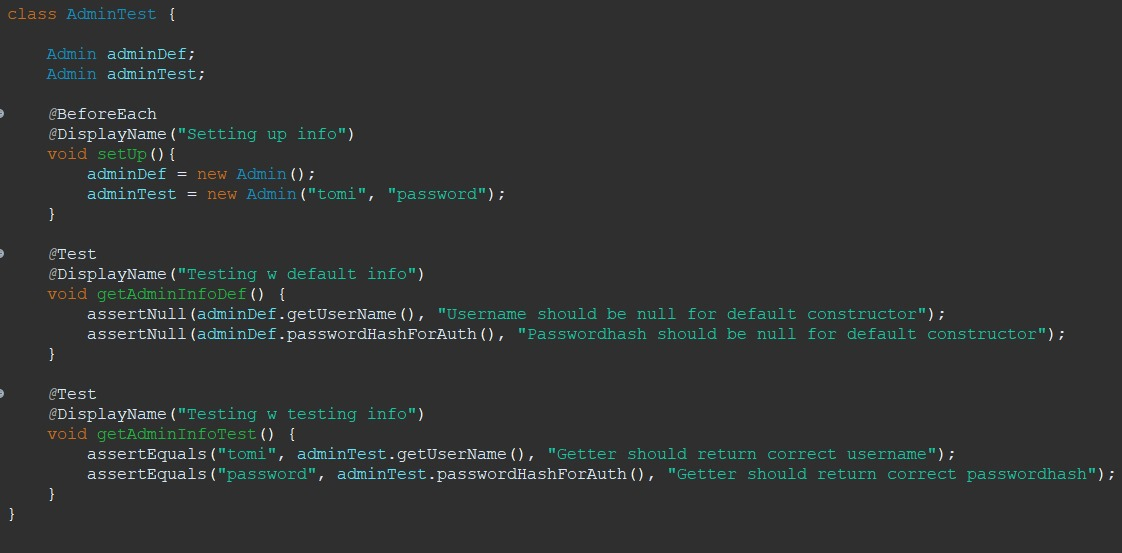
\includegraphics[width=\textwidth]{slike/adminTest.JPG}
				\caption{Kod klase AdminTest}
				\label{adminTest}
			\end{figure}
			
			Nadalje, provedeno je ispitivanje klase \textit{Accommodation} koja obrađuje informacije o smještaju u sustavu. Na donjoj slici prikazan je izvorni kod klase \textit{AccommodationTest} koji se sastoji od funkcije \textbf{setUp} koji stvara potrebne informacije, testa \textbf{testGetDefault} koji ispituje inicijalizaciju te provjerava njezinu ispravnost, inicijalna vrijednost za svaki atribut treba biti \textbf{NULL}. Test \textbf{testGetCorrect} testira stvaranje objekta kada su mu zadane neke vrjednosti, npr. adresa je \textit{address = Unska ulica 23, Zagreb}, tip smještaja je \textit{accommodationType = stan, 200}, broj zvjezdica je \textit{noOfStars = 3} i broj kreveta \textit{noOfBeds = 5} te povrat i spremanje danih vrijednosti.
			
			\begin{figure}[H]
				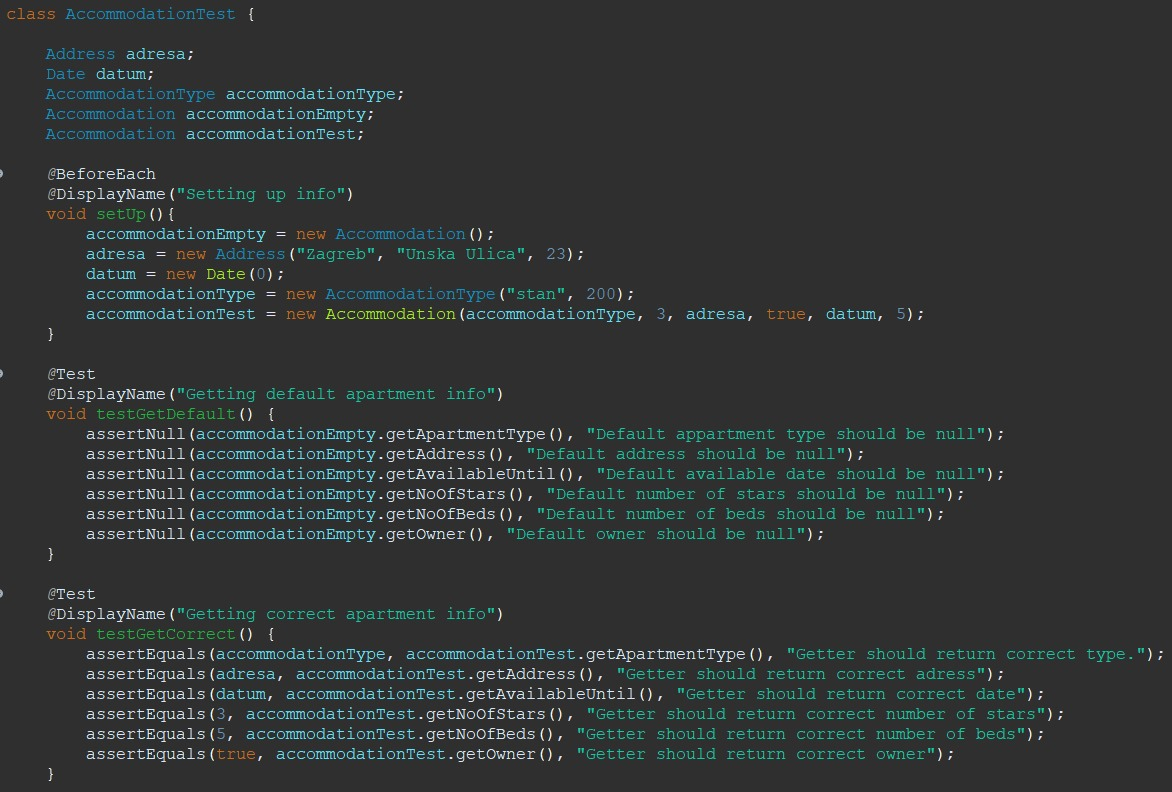
\includegraphics[width=\textwidth]{slike/AccommodationTest.JPG}
				\caption{Kod klase AccommodationTest}
				\label{AccommodationTest}
			\end{figure}
			
			Za kraj provedeno je ispitivanje klase \textit{UserTreatmentInfo}, na isti način kao i prethodne dvije klase, testiran je konstruktor bez zadanih vrijednosti i sa zadanim vrijednostima, jedina razlika je u tome da ova klasa ima dva konstruktora koji traže vrijednosti. Prvo inicijaliziramo tri insance klase \textbf{UserTreatmentInfo}, jedno bez zadanih vrijednosti, drugu u koju upisujemo vrijednosti: \textit{treatment\_id = 123L}, zatim za datum dolazka i odlaska isti, onaj koji jest u trenutku pokretanja, dalje za adresu dolaska i odlaska istu vrijednost \textit{address = "Zagreb, Savska, 132"}, istoga vozača na odlaku i povratku (čije vrijednosti su \textit{name="Marko", surname="Popić", \newline email="mail@mail.com", phoneNumber="0992583695"}, vozilo crveni \textit{Porcshe}, vrijeme početka rada trenutno, a za dane rada \textit{string="NUCP"}), smještaj s istim vrijednostima kao i u ispitivanju klase \textit{Accommodation}, datum usluge isti kao već spomenuti, trenutni (onaj u trenutku pokretanja testa) \textit{Timestamp} za trenutak zaključavanja i korisnik sa podacima \textit{name="Luke"}, \textit{surname="Skywalker"}, \newline \textit{email="lukeskywalker@force.com"}, \textit{phoneNumber = "036958721"} već spomenuti {accomodationType} te datum rođenja jednak onom pri pokretanju što se sprema u varjablu \textbf{userInfoTestOne}. Treći konstruktor traži samo tri vrijednosti datum liječenja što je u testnom primjeru postavljeno na jednak onom na dan testiranja, trenutak zaključavanja koji je postavljen na jednak način i korisnika usluge, on je postavljen jednako kao i u prethodnom konstruktoru, a sve je spremljeno u varijablu \textbf{userInfoTestToo}. Inicijalizaciju podataka pokazuje slika dolje.
			
			\begin{figure}[H]
				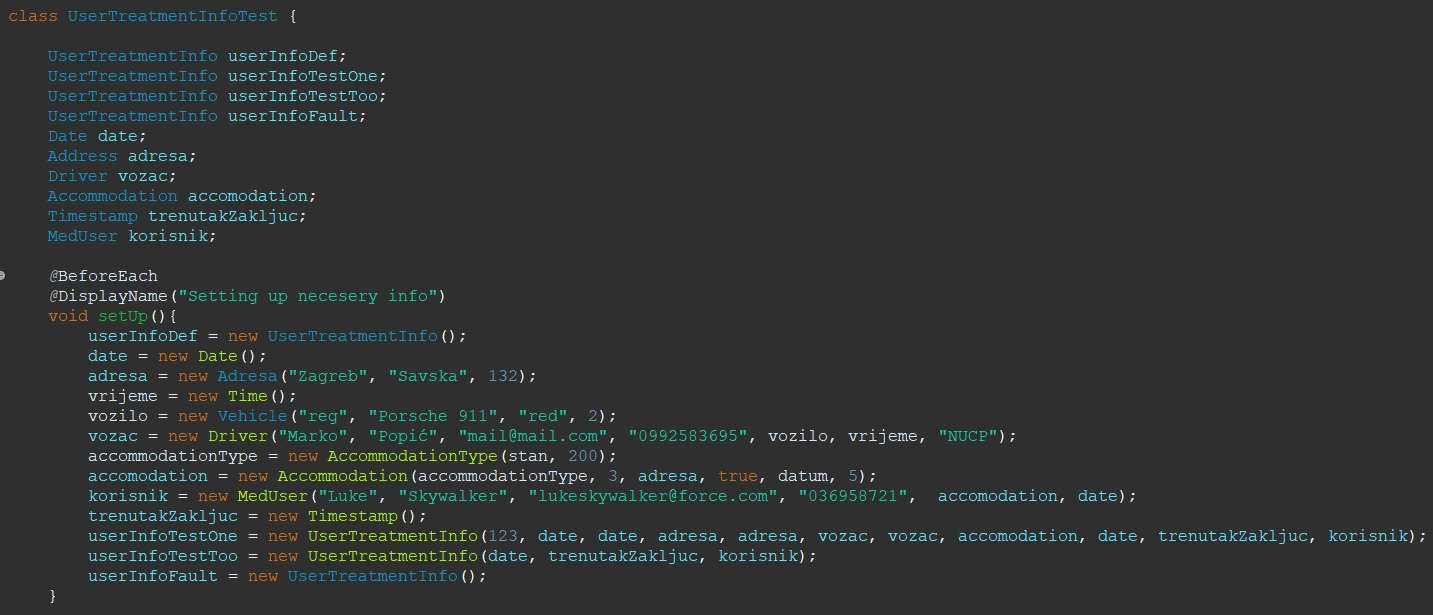
\includegraphics[width=\textwidth]{slike/userTreatmentInfoPtOne.JPG}
				\caption{Kod klase UserTreatmentTest, funkcija \textbf{setUp}}
				\label{UserTreatmentInfoTestPtOne}
			\end{figure}
			
			Konstruktor bez zadanih vrijednosti treba za svaki atribut postaviti \textbf{NULL} što provjerava test \textbf{getUserInfoDef}. Prvi konstruktor treba postaviti vrijednosti oblika varijable \textbf{userInfoTestOne} što provjerava test \textbf{getUserInfoOne} što je prikazano na slici dolje.
				
			\begin{figure}[H]
				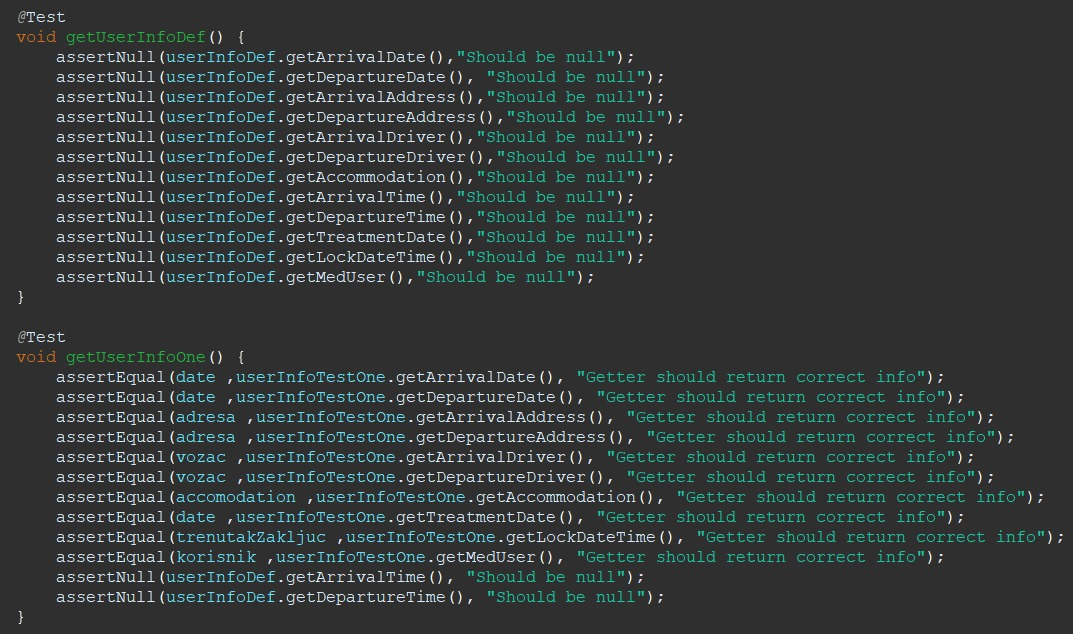
\includegraphics[width=\textwidth]{slike/userTreatmentInfoPtToo.JPG}
				\caption{Kod klase UserTreatmentTest, test \textbf{getUserInfoDef} i test \textbf{getUserInfoOne}}
				\label{UserTreatmentInfoTestPtToo}
			\end{figure}
			
			 Posljednji konstruktor prima vrijednosti oblika varijable  \textbf{userInfoTestToo}, a ispravnost postavljanja provjerava test \textbf{getUserInfoToo} čiji je izvorni kod prikazan na slici dolje.
			
			\begin{figure}[H]
				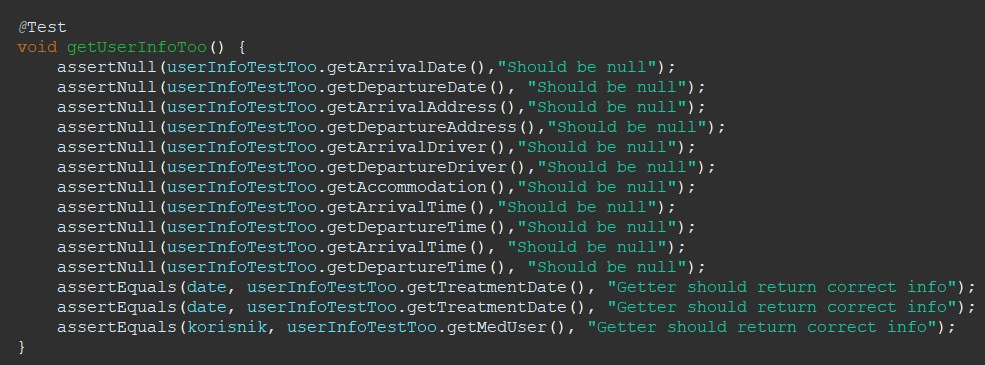
\includegraphics[width=\textwidth]{slike/userTreatmentInfoPtTree.JPG}
				\caption{Kod klase UserTreatmentTest, test \textbf{getUserInfoToo}}
				\label{UserTreatmentInfoTestPtTree}
			\end{figure}
			
			\subsection{Ispitivanje sustava}
			
			 %\textit{Potrebno je provesti i opisati ispitivanje sustava koristeći radni okvir Selenium\footnote{\url{https://www.seleniumhq.org/}}. Razraditi \textbf{minimalno 4 ispitna slučaja} u kojima će se ispitati redovni slučajevi, rubni uvjeti te poziv funkcionalnosti koja nije implementirana/izaziva pogrešku kako bi se vidjelo na koji način sustav reagira kada nešto nije u potpunosti ostvareno. Ispitni slučaj se treba sastojati od ulaza (npr. korisničko ime i lozinka), očekivanog izlaza ili rezultata, koraka ispitivanja i dobivenog izlaza ili rezultata.\\ }
			 
			 %\textit{Izradu ispitnih slučajeva pomoću radnog okvira Selenium moguće je provesti pomoću jednog od sljedeća dva alata:}
			 %\begin{itemize}
			 %	\item \textit{dodatak za preglednik \textbf{Selenium IDE} - snimanje korisnikovih akcija radi automatskog ponavljanja ispita}
			 %	\item \textit{\textbf{Selenium WebDriver} - podrška za pisanje ispita u jezicima Java, C\#, PHP koristeći posebno programsko sučelje.}
			 %\end{itemize}
		 	%\textit{Detalji o korištenju alata Selenium bit će prikazani na posebnom predavanju tijekom semestra.}
			
			Zbog broja ne implementiranih funkcija na sustavu testiranje je ograničeno. \newline
			Provjerava se dodavanje novog korisnika (\textit{user}), vozača (\textit{driver}), administratora (\textit{admin}) te smještaja (\textit{accommodation}).
			Za početak, dodavanje novog korisnika nije moguće preko tipke koja je za tu funkciju predviđena. Očekivani rezultat bi bio prikaz dodanog korisnika, ali korisnik se ne dodaje te ne prikazuje.
			
			\begin{figure}[H]
				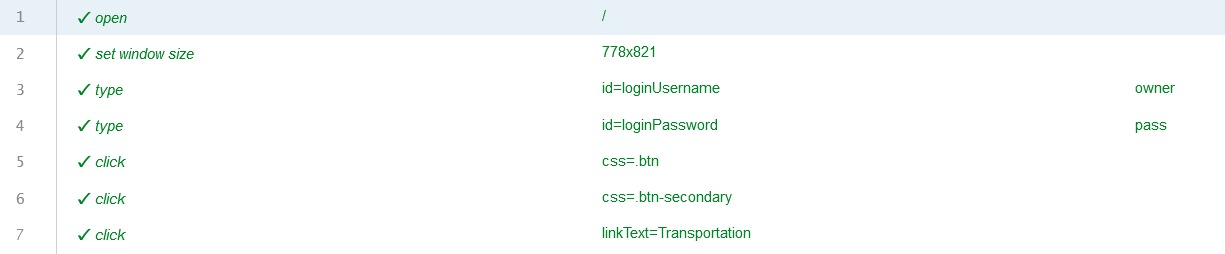
\includegraphics[width=\textwidth]{slike/addingANewUserTest.JPG}
				\caption{Snimka kako bi dodavanje novog korisnika trebalo izgledati}
				\label{addingANewUserTest}
			\end{figure}
			
			\begin{figure}[H]
				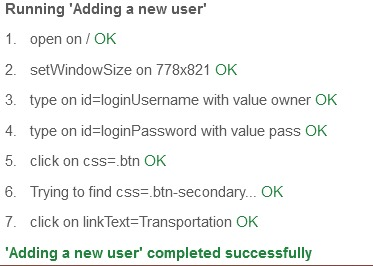
\includegraphics[width=\textwidth]{slike/addingANewUserResults.JPG}
				\caption{Rezultati testa}
				\label{addingANewUserResults}
			\end{figure}
			
			Nadalje, klik na gumb za koji je predviđeno dodavanje novog vozača otvara formu predviđenu za to. Nakon upisa podataka i klika na gumb za dodati novog vozača, novi vozač bi se trebao prikazati u listi, ali to se ne događa.
			
			\begin{figure}[H]
				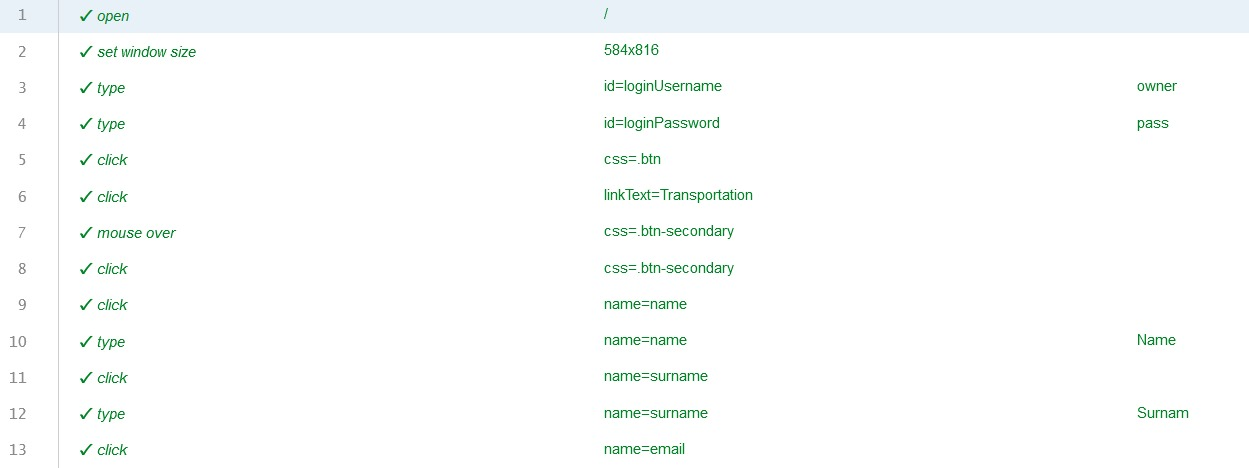
\includegraphics[width=\textwidth]{slike/addingANewDriverTest.JPG}
				\caption{Snimka kako bi dodavanje novog vozača trebalo izgledati}
				\label{addingANewDriverTest}
			\end{figure}
			
			\begin{figure}[H]
				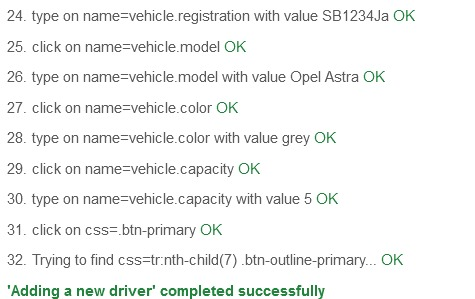
\includegraphics[width=\textwidth]{slike/addingANewDriverResults.JPG}
				\caption{Rezultati testa}
				\label{addingANewDriverResults}
			\end{figure}
			
			Treći test je dodavanje novog administratora, pri pritsku na tipku koja je za to predviđena otvara se forma koja omogućuje upis novog administratora, ali on se ne prikazuje, kao ni jedan upisani adminstrator u sustavu.
			
			\begin{figure}[H]
				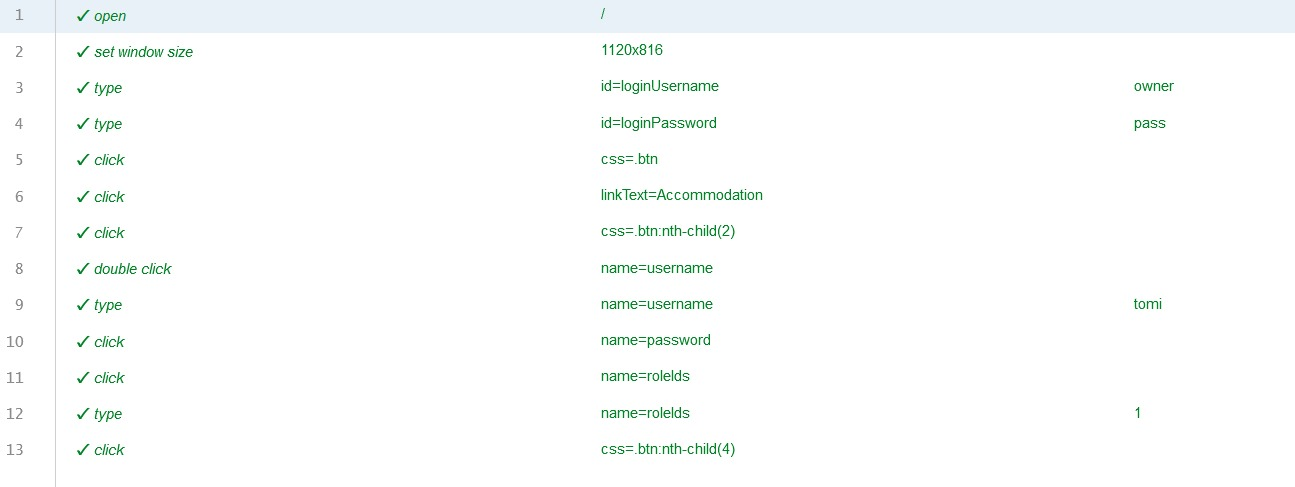
\includegraphics[width=\textwidth]{slike/addingANewAdminTest.JPG}
				\caption{Snimka kako bi dodavanje novog korisnika trebalo izgledati}
				\label{addingANewAdminTest}
			\end{figure}
			
			\begin{figure}[H]
				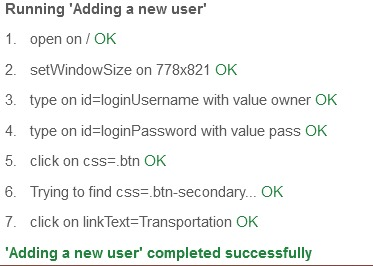
\includegraphics[width=\textwidth]{slike/addingANewUserResults.JPG}
				\caption{Rezultati testa}
				\label{addingANewAdinResults}
			\end{figure}
			
			Posljednji test je dodavanje novog smještaja, pri pritisku na tipku koja je zato predviđena otvara se forma koja omogućuje upis novog smještaja, ali on se ne prikazuje s ostalim, već upisanim smještajima.
			
			\begin{figure}[H]
				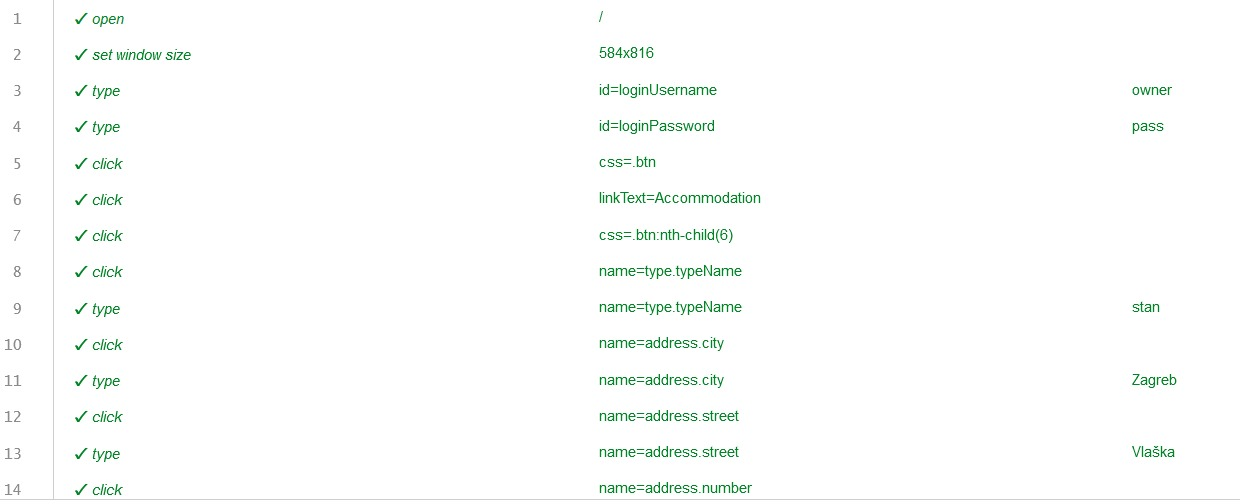
\includegraphics[width=\textwidth]{slike/addingANewAccTest.JPG}
				\caption{Snimka kako bi dodavanje novog smještaja trebalo izgledati}
				\label{addingANewAccTest}
			\end{figure}
			
			\begin{figure}[H]
				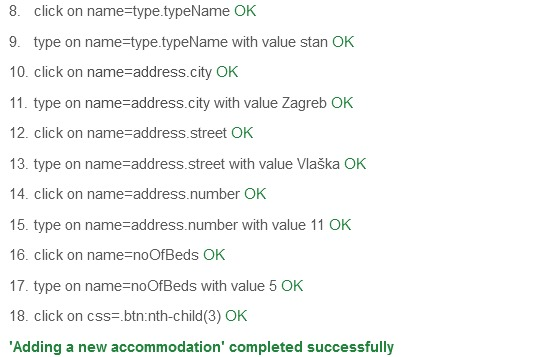
\includegraphics[width=\textwidth]{slike/addingANewAccResults.JPG}
				\caption{Rezultati testa}
				\label{addingANewAccResults}
			\end{figure}
			
			Testiranje sustava pokazuje da on nije u mogućnosti ostvariti komunikaciju između frontenda i backenda, ali da je u mogućnosti prikazati prethodno upisane vrijednosti u bazi podataka. 
			
			\eject 
		
		
		\section{Dijagram razmještaja}

		{Na slici prikazan je dijagram razmještaja. Cjelokupan sustav je baziran na arhitekturi "klijent-poslužitelj". Klijentsko računalo i poslužitelj za frontend povezani su protokolom HTTP. Na poslužiteljskom računalu nalaze se Frontent-react, Backend-Spring i DB poslužitelj. Spring iz backenda dohvaća podatke iz SQL baze podataka.}
			
		\begin{figure}[H]
			\includegraphics[width=\linewidth]{slike/Dijagram razmještaja.JPG}
			\centering
			\caption{Dijagram razmještaja}
			\label{fig:Dijagram razmještaja}
		\end{figure}
		\eject 
		
		\section{Upute za puštanje u pogon}
		
			%\textbf{\textit{dio 2. revizije}}\\
		
			 %\textit{U ovom poglavlju potrebno je dati upute za puštanje u pogon (engl. deployment) ostvarene aplikacije. Na primjer, za web aplikacije, opisati postupak kojim se od izvornog kôda dolazi do potpuno postavljene baze podataka i poslužitelja koji odgovara na upite korisnika. Za mobilnu aplikaciju, postupak kojim se aplikacija izgradi, te postavi na neku od trgovina. Za stolnu (engl. desktop) aplikaciju, postupak kojim se aplikacija instalira na računalo. Ukoliko mobilne i stolne aplikacije komuniciraju s poslužiteljem i/ili bazom podataka, opisati i postupak njihovog postavljanja. Pri izradi uputa preporučuje se \textbf{naglasiti korake instalacije uporabom natuknica} te koristiti što je više moguće \textbf{slike ekrana} (engl. screenshots) kako bi upute bile jasne i jednostavne za slijediti.}
			Upute za puštanje u pogon su podijeljene u tri dijela jer svaki od tri dijela aplikacije (frontend, backend, baza podataka) zahtjeva posebnu pripremu za postavljanje na server.
			Početni koraci su jednaki za sve komponente, potrebno je prijaviti se na \url{https://render.com/} (u slučaju prvog korištenja registrirati se) te na izborniku kao na slici odabrati što se želi pustiti u pogon.
			\begin{figure}[H]
				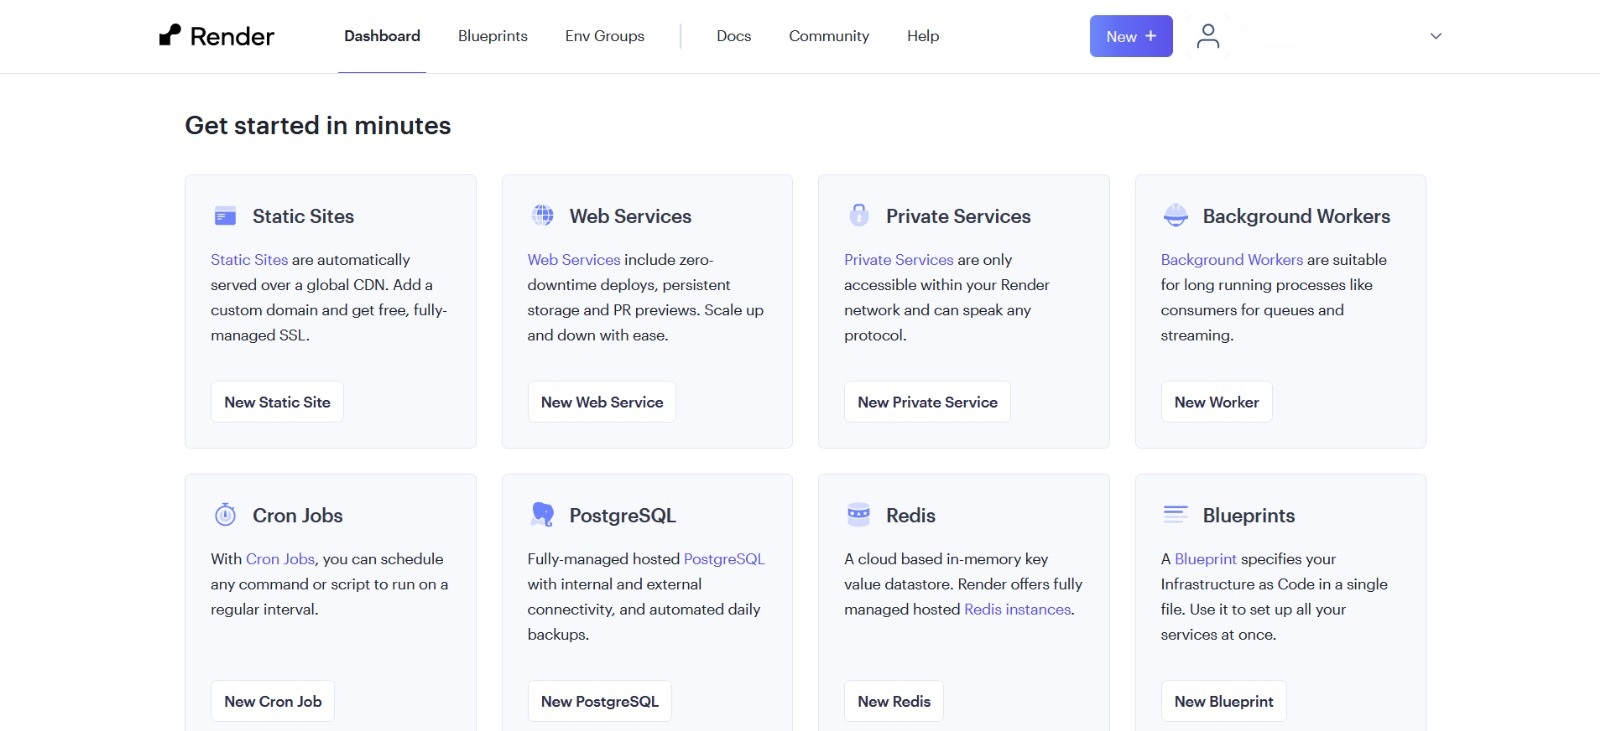
\includegraphics[width=\linewidth]{slike/RenderIzbornik.JPG}
				\centering
				\caption{Izbornik sustava za puštanje u pogon na Renderu}
				\label{fig:Izbornik Render}
			\end{figure}
			\textbf{Baza podataka} \newline
			Puštanje u pogon započinje postavljanjem baze podataka, to činimo odabirom opcije \textbf{New PostgreSQL} u izborniku. Taj odabir će otvoriti prozor prikazan na slici.
			\begin{figure}[H]
				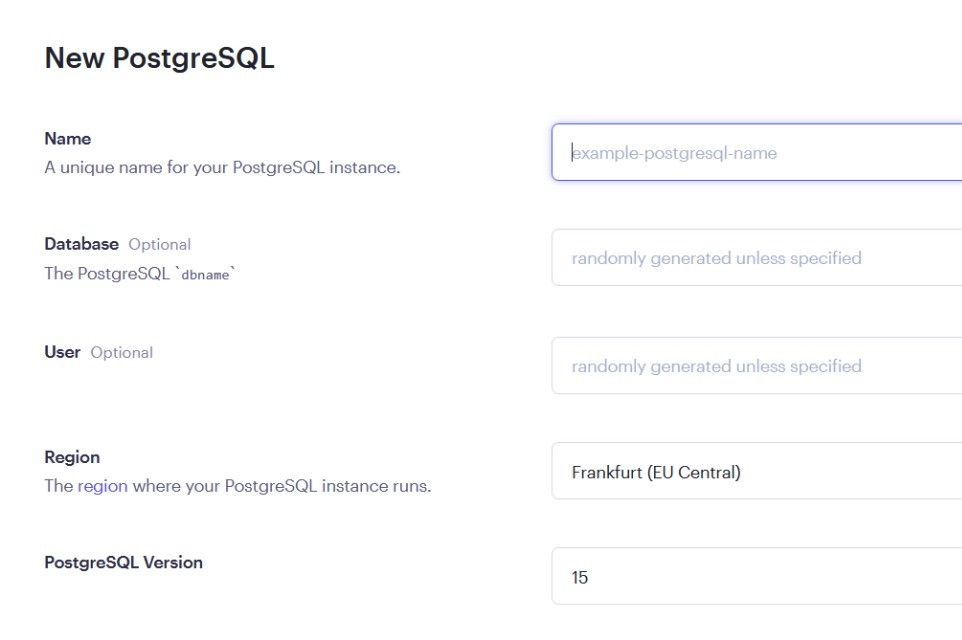
\includegraphics[width=\linewidth]{slike/PostgreSQLprviDio.JPG}
				\centering
				\caption{Izgled izbornika za puštanje baze podataka u pogon.}
				\label{fig:PostgreSQL izbornik prvi dio}
			\end{figure}
			Za puštanje u pogon, potrebno je iz izbornika za regiju (\textit{Region}) odabrati opciju Frankfurt, upisati ime baze podataka (npr. Error404-DentAll-BazaPodataka) u polje \textit{Name} što se može vidjeti na slici iznad. Zatim odabrati besplatnu opciju u izborniku tipa (\textit{Instance type}), prikazano na slici dolje. Naposljetku je potrebno pritisnuti gumb "\textit{Create Database}" također prikazan na slici dolje. Sva ostala polja mogu ostati prazna.
			\begin{figure}[H]
				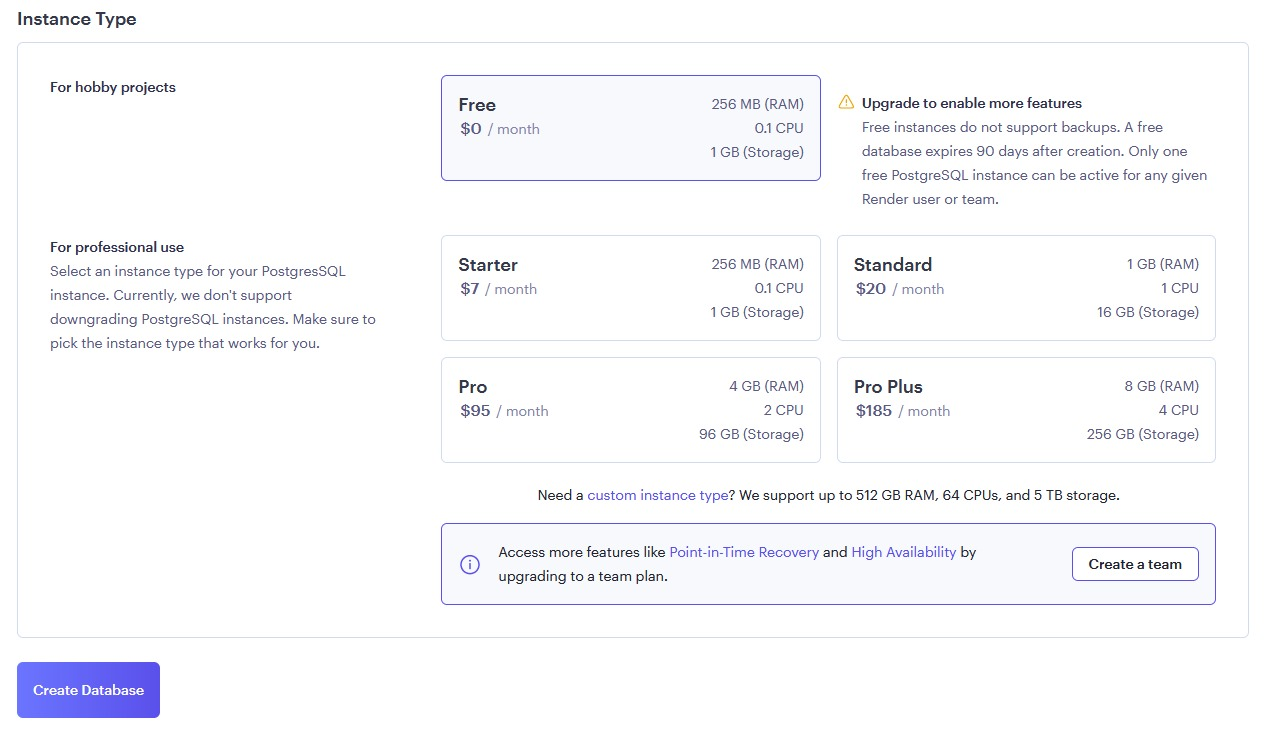
\includegraphics[width=\linewidth]{slike/PostgreSQLdrugiDio.JPG}
				\centering
				\caption{Izgled izbornika za puštanje baze podataka u pogon.}
				\label{fig:PostgreSQL izbornik drugi dio}
			\end{figure}
			\textbf{Frontend i Backend} \newline
			Puštanje u pogon frontenda i backenda započinje jednako, odabirom opcije \textbf{New Web Service} u već prikazanom izborniku. Zatim je potrebno povezati vlastiti GitHub račun sa Renderom te upisati url repozitorija (upisati \url{https://github.com/Tomislav-Pranjic/Error404-DentAll} u prostor za javne repozitorije) prikazano na donjoj slici.
			\begin{figure}[H]
				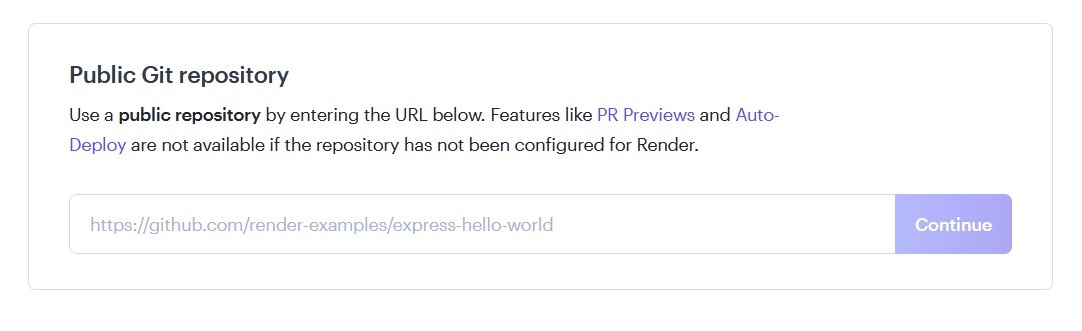
\includegraphics[width=\linewidth]{slike/PublicRepo.JPG}
				\centering
				\caption{Mjesto za upis URL-a mape u kojoj se nalazi web servis}
				\label{fig:Izbornik za puštanje web servisa}
			\end{figure}
			Za početak će biti opisano puštanje u pogon backenda. \newline
			\textbf{1. korak} \newline 
			Prvo ćemo odabrati ime web servisa, primjer "Error404-be", zatim odabrati istu regiju kao i za bazu podataka (Frankfurt), nadalje potrebno je odabrati granu koda sa koje puštamo backend u pogon, ime grane je "main", onda je potrebno upisati korijensku mapu (\textit{IzvorniKod/error404-be}), te konačno od raznih vrsta web servisa potrebno odabrati pravi \textit{Runtime}, za Backend je to \textbf{Docker}, kako prozor izgleda na kraju ovog koraka vidi se na slici.
			\begin{figure}[H]
				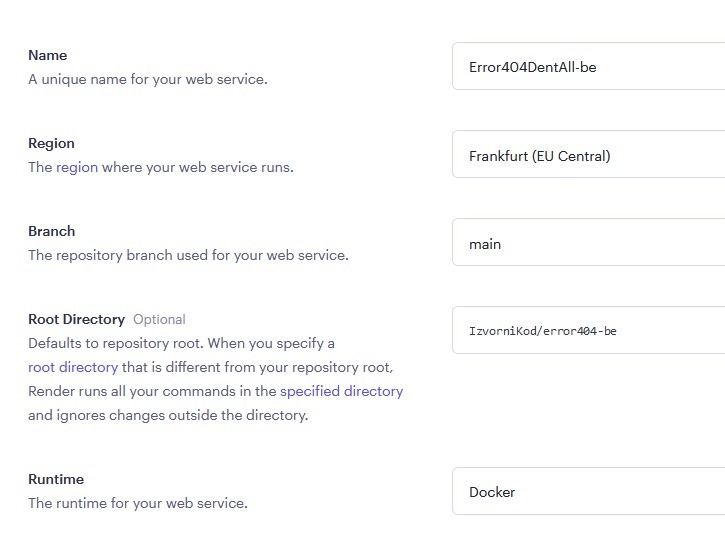
\includegraphics[width=\linewidth]{slike/BackendPtOne.JPG}
				\centering
				\caption{Mjesto za odabira imena, regije, grane, mape te vrste web servisa}
				\label{fig:Backend prvi}
			\end{figure}
			\textbf{2. korak} \newline U ovom koraku odabiremo besplatnu verziju tipa servera (\textit{Instance type}), isto kao i kod baze podataka, zatim stvaramo dvije varijable okoline \newline \textit{OWNER\_PASS = "\$2a\$10\$6djQ3MpO06d5dgvp9ijBee6ZKKj5L5iJVrrDPQjtD4I6em2p7JjMu"}, i \textit{PORT = 8080},
			koje će služiti kako bismo mogli povezati backend i frontend.
			\begin{figure}[H]
				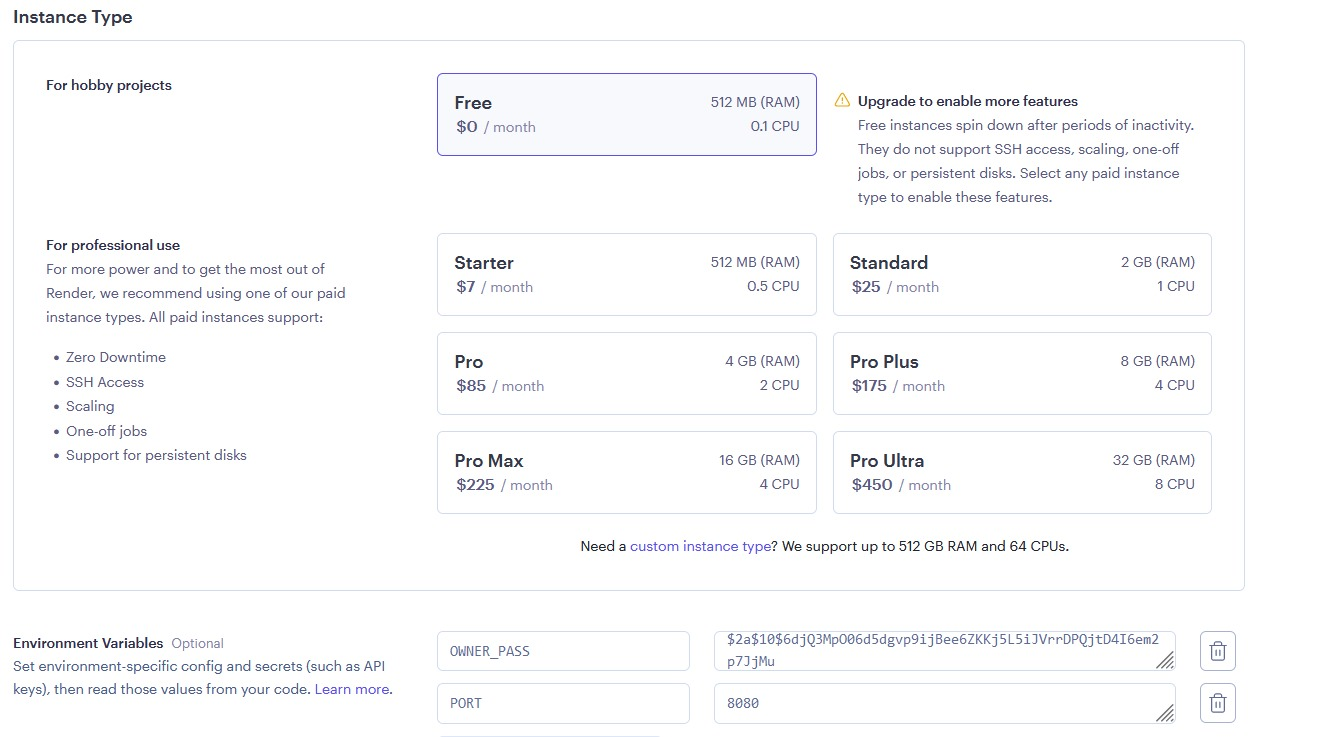
\includegraphics[width=\linewidth]{slike/BackendPtToo.JPG}
				\centering
				\caption{Mjesto za odabira tipa, i upis varijabli okoline}
				\label{fig:Backend drugi}
			\end{figure}
			\textbf{3. korak} \newline Dalje odabiremo opciju \textit{Advanced} koja nam dopušta dodatne opcije uređivanja poput specificiranja \textit{Health Check Path}, stranice koja će uvijek vraćati HTTP kod "200 OK", a služi za provjera rada backend-a.
			\begin{figure}[H]
				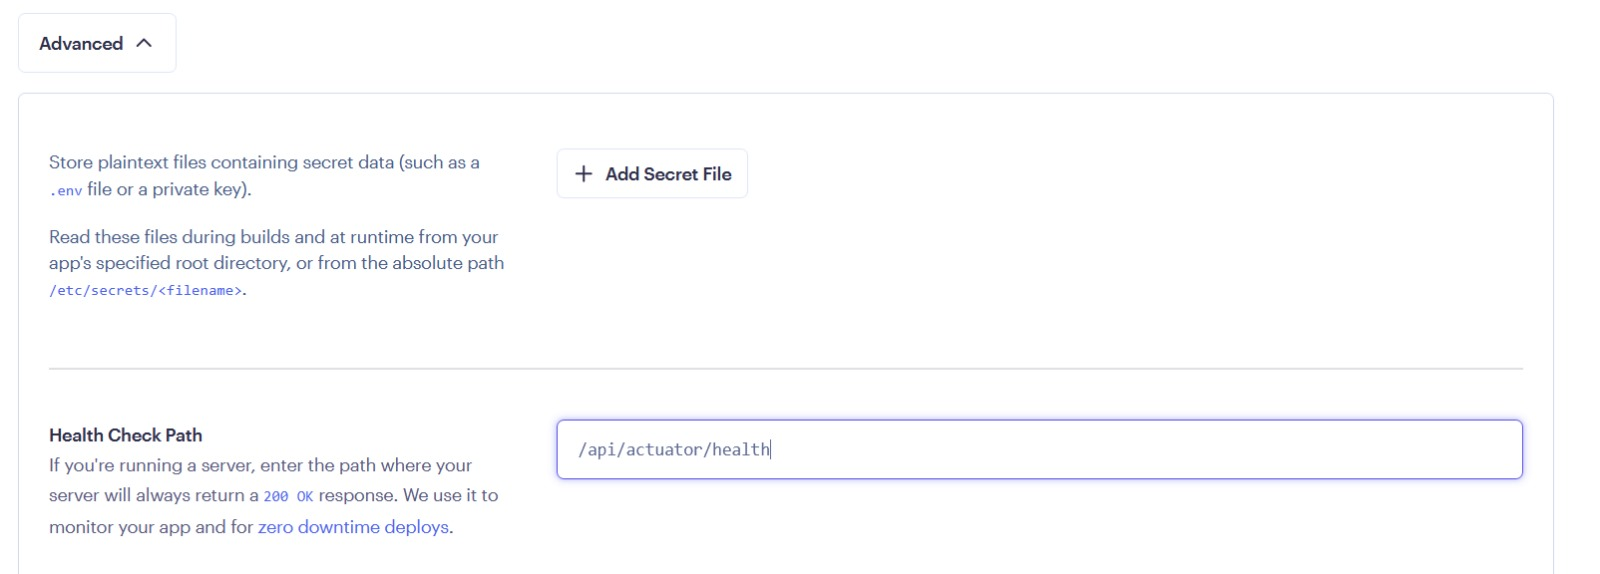
\includegraphics[width=\linewidth]{slike/BackendPtTree.JPG}
				\centering
				\caption{Mjesto za specificiranja Health Check puta}
				\label{fig:Backend treći}
			\end{figure}
			\textbf{4. korak} \newline Dalje, potrebno je upisati lokaciju \textit{Docerfile-a}, relativno korijenskoj mapi (\textit{/docker/maven/Dockerfile}), te konačno pritisnuti gumb \textbf{Create Web Service}, ostale postavke ostaviti kako su inicijalizirane.
			\begin{figure}[H]
				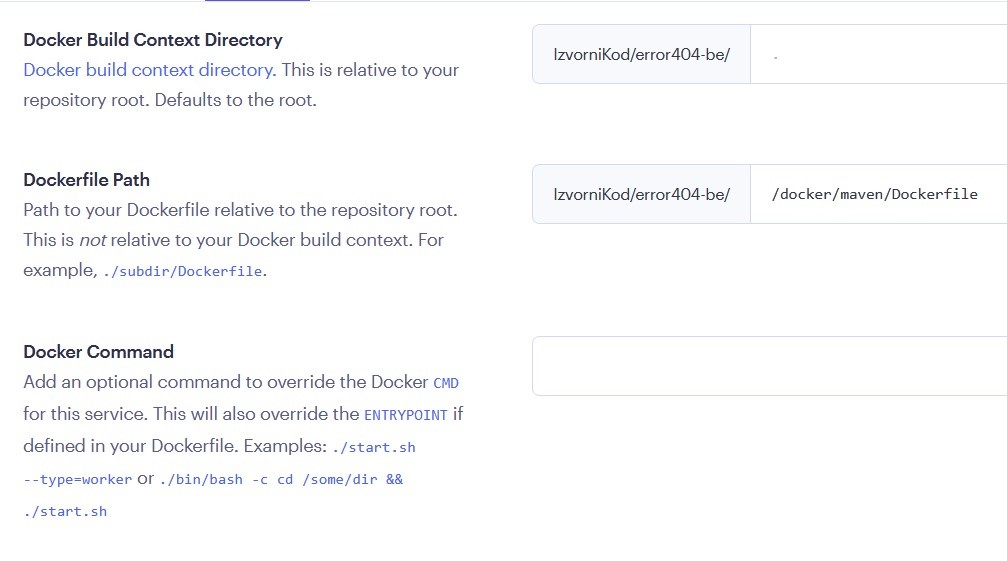
\includegraphics[width=\linewidth]{slike/BackendPtFor.JPG}
				\centering
				\caption{Mjesto za specificiranja docerfile lokacije}
				\label{fig:Backend četvrti}
			\end{figure}
			\begin{figure}[H]
				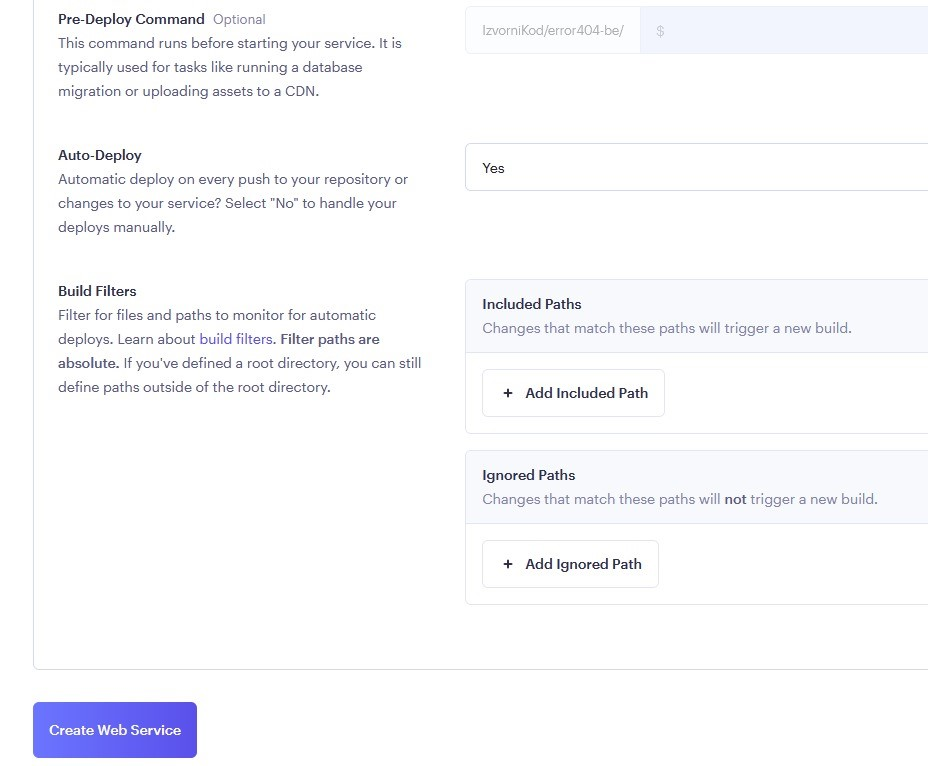
\includegraphics[width=\linewidth]{slike/BackendPtV.JPG}
				\centering
				\caption{Gumb za stvaranje web servisa}
				\label{fig:Backend peti}
			\end{figure}
			Dalje će biti opisan postupak puštanja frontenda u pogon.  %Abandon all hope, ye who enter here
			\newline 
			\textbf{1. korak} \newline
			Za početak, kao i svagdje, odabiremo ime servisa, neka to za primjer bude "Error404-DentAll-fe", zatim odabiremo već poznatu regiju (Frankfurt), te istu granu kao i za backend ("main"), korijenska mapa ovoga je puta \textit{IzvorniKod/error404-fe} te se upisuje na isto mjesto kao i kod backenda, ali za razliku od backenda, \textit{Runtime} je \textbf{Node}. Kao \textit{Build Command} upisujemo \textbf{yarn build}, a kao \textit{Start Command} \textbf{yarn start-prod}.
			\begin{figure}[H]
				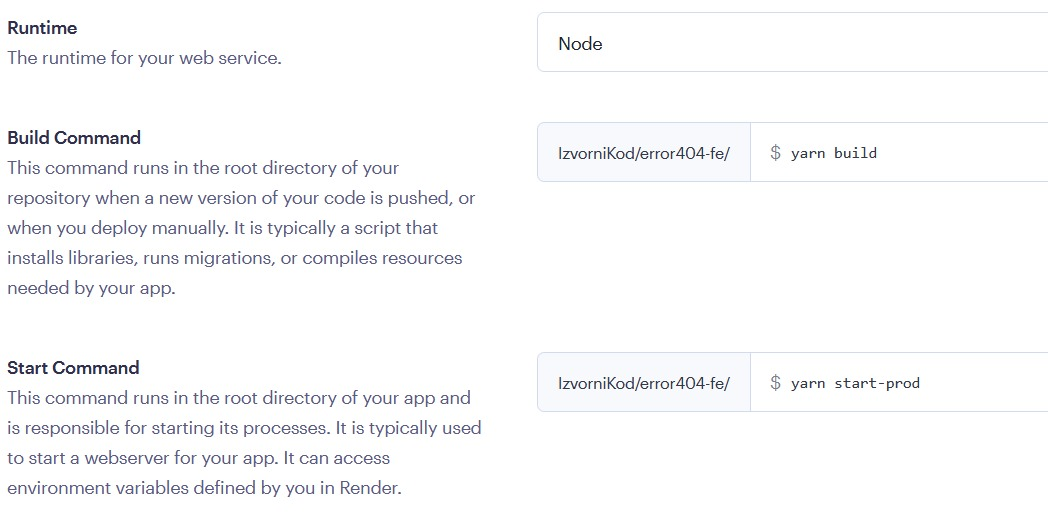
\includegraphics[width=\linewidth]{slike/FrontendPtOne.JPG}
				\centering
				\caption{Konfiguracija frontenda}
				\label{fig:Frontend prvi}
			\end{figure}
			\textbf{2. korak} \newline
			Za razliku od backenda ne koristimo nikakve proširene mogućnosti nego samo stvaramo 2 varijable okoline, \textit{API\_URL = "https://error404dentall-be.onrender.com/api"}, i \textit{PORT = 8080},
			koje će služiti kako bismo mogli povezati frontend i backend. Nakon toga jednostavno se pritisne gumb \textbf{Create Web Service} i novi servis je stvoren.
			\begin{figure}[H]
				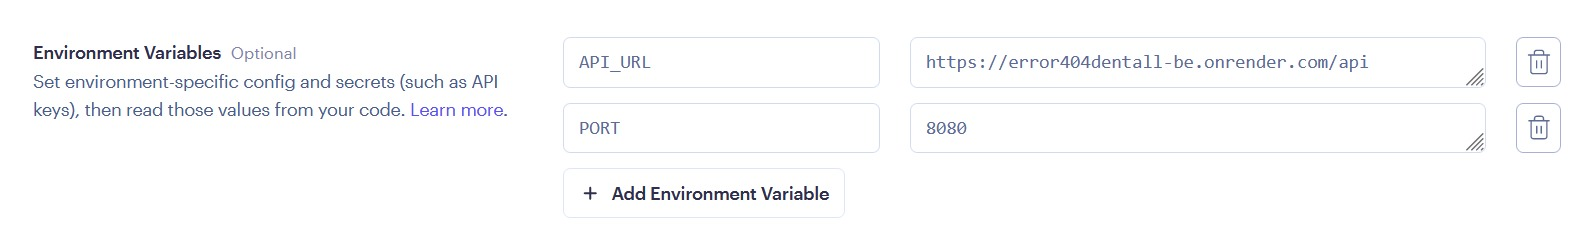
\includegraphics[width=\linewidth]{slike/FrontendPtToo.JPG}
				\centering
				\caption{Konfiguracija varijabli okoline}
				\label{fig:Frontend drugi}
			\end{figure}
			 %\textit{Dovršenu aplikaciju potrebno je pokrenuti na javno dostupnom poslužitelju. Studentima se preporuča korištenje neke od sljedećih besplatnih usluga: \href{https://aws.amazon.com/}{Amazon AWS}, \href{https://azure.microsoft.com/en-us/}{Microsoft Azure} ili \href{https://www.heroku.com/}{Heroku}. Mobilne aplikacije trebaju biti objavljene na F-Droid, Google Play ili Amazon App trgovini.}
			
			
			\eject 
